\section{Machine learning model evaluation}

This chapter evaluates the predictive performance of my machine learning model.
The model's forecasts are benchmarked against both actual sensor data and the
predictions from a simpler alternative model, before discussing the results.

\subsection{Models being compared}

The three models that I compared against the actual sensor readings are included
below.

\begin{enumerate}
    \item{General forecast weather from OpenWeather} 
    \item{Proposed machine learning model (Chapter \ref{sec:machine-learning})} 
    \item{Alternative model - an adjusted version of the OpenWeather using a mean average adjustment}
\end{enumerate}

\subsection{Procedure}

To evaluate the models I compared the results from all three models over the
same 48 hour period (which is the limit of the OpenWeather forecast). The
measurements started at 00:00 on Saturday, 30 August 2025, and concluded at
23:00 on Sunday, 31 August 2025. 

The OpenWeather forecast and machine learning prediction were collected
automatically by my backend (using node\_cron and endpoints, see Section
\ref{sec:building-api}) and stored in a temporary database table I made
specifically for this evaluation.

The alternative model was made by comparing the average temperature, humidity
and wind speed differences between my raw sensor data and OpenWeather current
weather readings from my database. To make the comparison fair with the machine
learning model, I used data from 15--27 August (the same as the ML's training
data) so that the alternative model would not have a larger amount of data. The
purpose of including the alternative model was to assess whether a simple bias
correction model was any different to my more complex machine learning
procedure.

\subsection{Charts and results}

As the weather data for the selected period was very similar between both nodes
I have decided to only show charts for node 1 as it is representative of node 2
as well. I have included a table containing the Mean Absolute Error (MAE) and
Root Mean Squared Error (RMSE) for the data in these charts in Appendix
\ref{app:ml-stats}.

\begin{figure}[H]
    \centering
    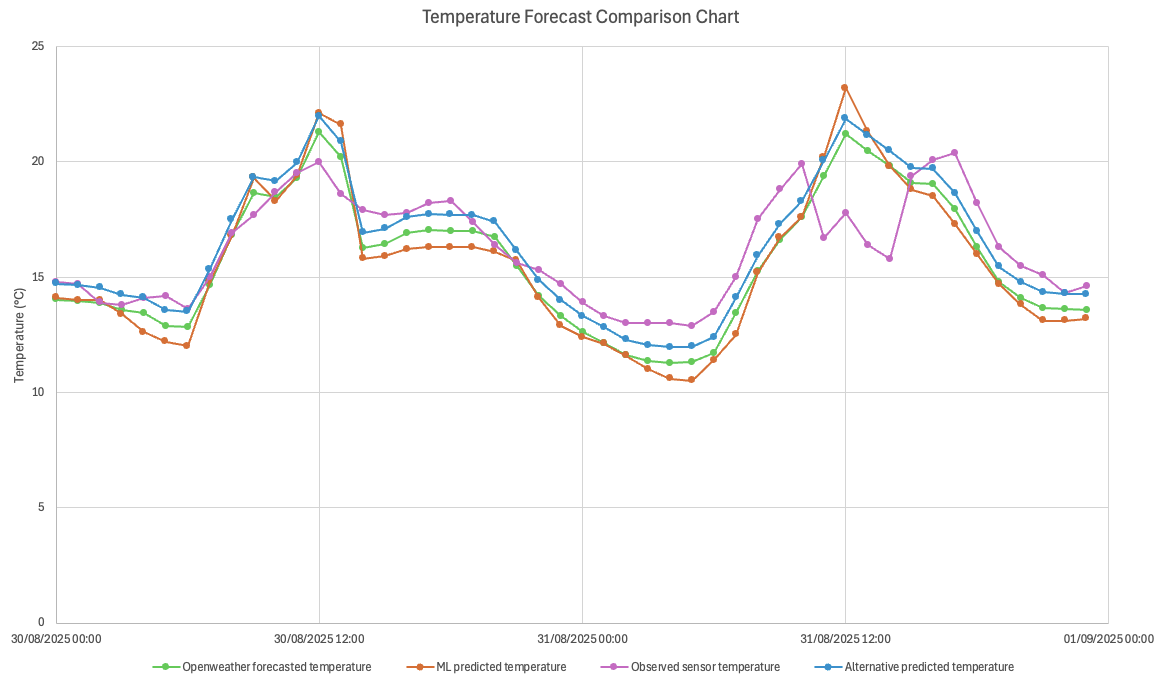
\includegraphics[width=0.95\textwidth]{contents/part-4/fig4/temperature-graph.png}
    \caption{Chart comparing temperature forecast models}
    \label{fig:temperature-chart}
\end{figure}

Figure \ref{fig:temperature-chart} shows that the machine learning model
(orange) does not appear to track particularly close to the observed figures
(pink). The relative MAE (see Appendix \ref{app:ml-stats}) of the machine
learning model here is 2.9\% while the general forecast is only slightly higher
at 3.4\%\footnote{MAE scores to be interpreted as so: a higher score means that
the error compared to the actual sensor reading was greater. A lower score
indicates a closer (better) relationship}, meaning the ML model is only
marginally better than its training data at predicting temperature. The
alternative model performs better with an MAE of 1.3\%. Both the ML and
alternative models predicted a higher peak temperature on both days than either
the sensor data or the forecast, suggesting that the data from 15th - 27th
August may not have been a representative sample and is biased towards higher
temperatures.

\begin{figure}[H]
    \centering
    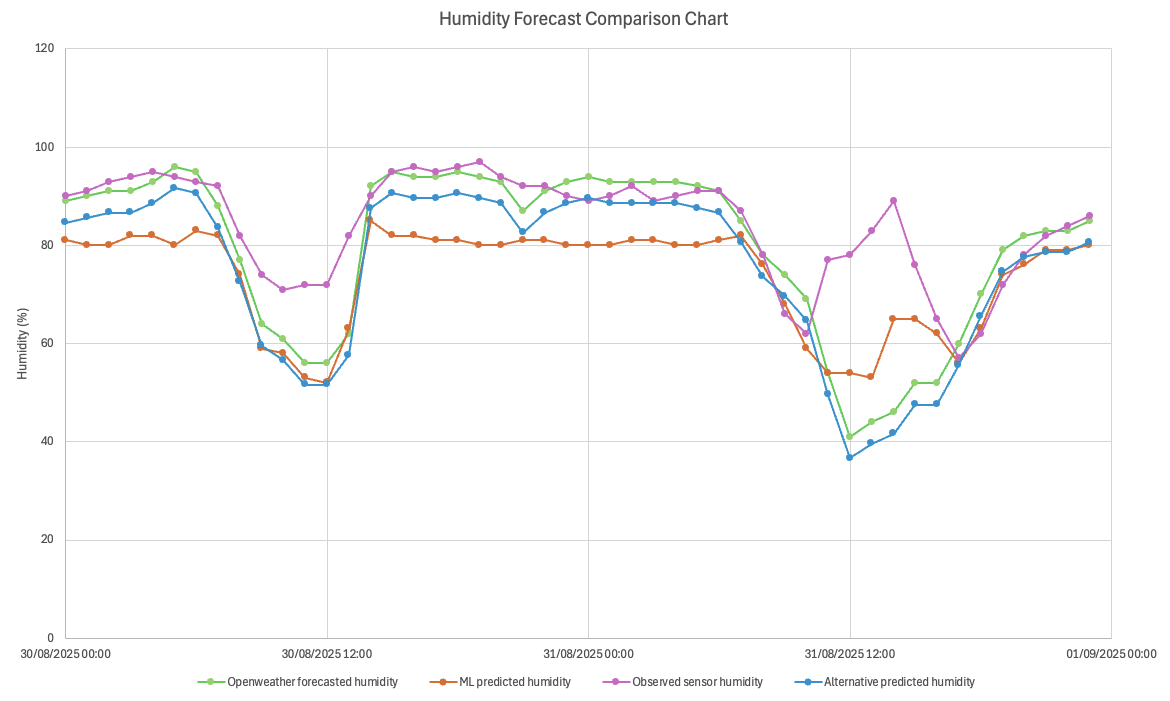
\includegraphics[width=1\textwidth]{contents/part-4/fig4/humidity-graph.png}
    \caption{Chart comparing humidity forecast models}
    \label{fig:humidity-chart}
\end{figure}

In Figure \ref{fig:temperature-chart} the machine learning model performed
particularly poorly on average with an MAE OF 14.9\% (General forecast: 5.5\%).
The alternative model also performs worse with MAE of 11.1\%. While these
metrics paint a poor picture of the model, I would point to the section of the
chart around 12:00 31/08. Here we can see that the machine learning model is the
only one of hte models to successfully predict a spike in humidity at midday.
While the magnitude of this spike is not correct it does offer some tentative
evidence that the model has some predictive power on the microclimate that the
general weather cannot pick up.

\begin{figure}[H]
    \centering
    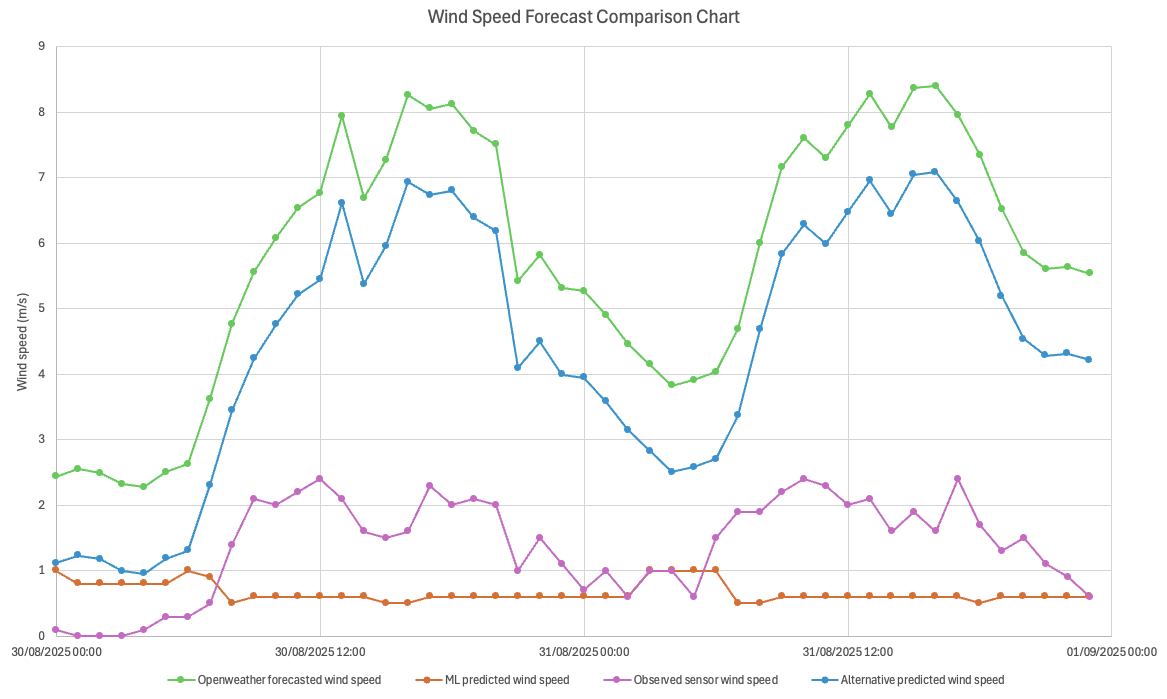
\includegraphics[width=1\textwidth]{contents/part-4/fig4/wind-speed-graph.png}
    \caption{Chart comparing wind speed forecast models}
    \label{fig:wind-chart}
\end{figure}

With wind speed the ML model performs better relative to the either the general
forecast or the adjusted forecast used in the alternative model. This is
reflected in an MAE of 43.6\% for the machine learning model versus 381.9\% and
264\% for the general forecast and alternative model respectively.

\begin{figure}[H]
    \centering
    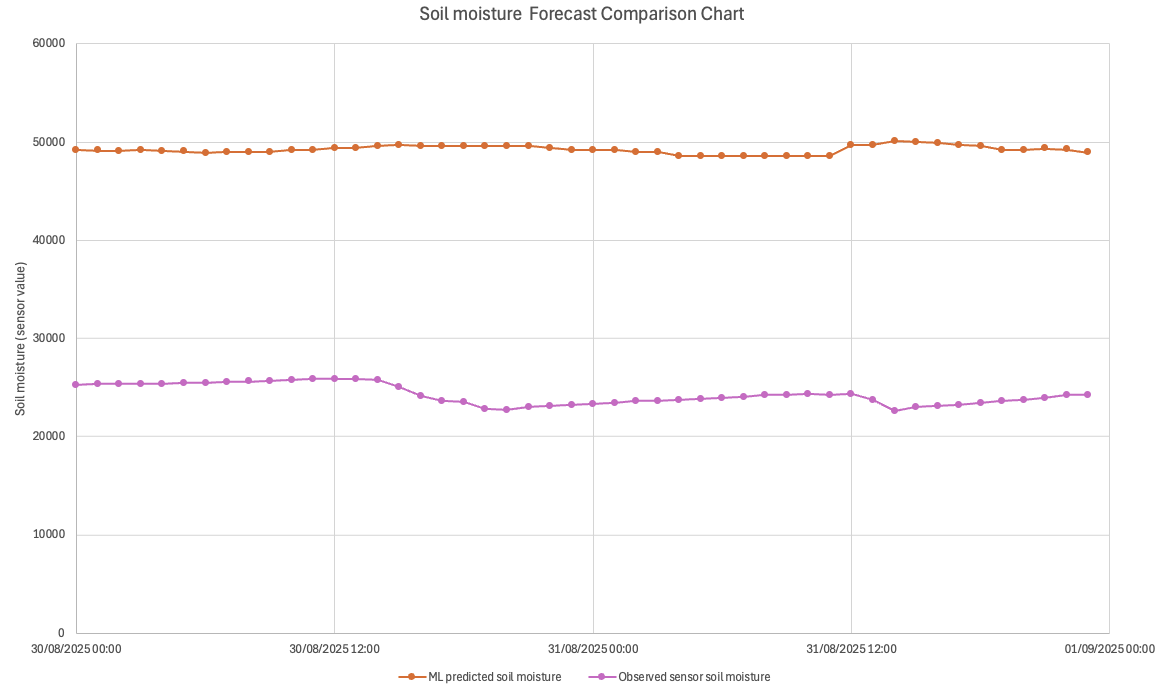
\includegraphics[width=1\textwidth]{contents/part-4/fig4/soil-graph.png}
    \caption{Chart comparing soil moisture predicted by machine learning model versus actual readings}
    \label{fig:soil-chart}
\end{figure}

\subsection{Discussion of results}
